\begin{figure}[htbp]
\centering
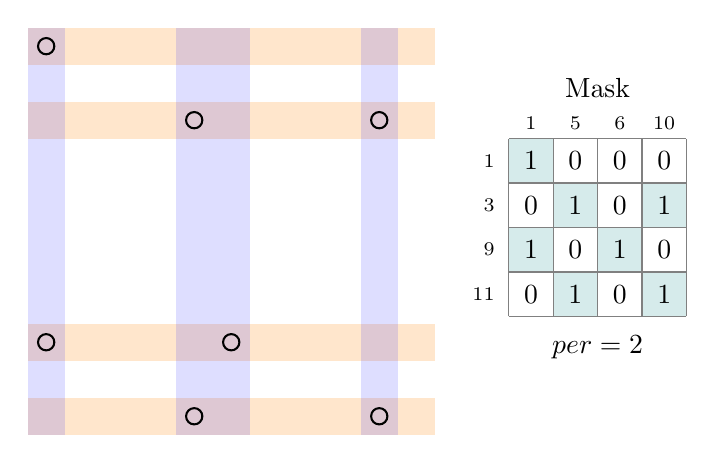
\begin{tikzpicture}[x=.47cm,y=.47cm]
 \bcuadricula{11}
 \foreach \rr in {1,3,9,11}{\fill[orange,opacity=.20] (0,{11-\rr}) rectangle (11,{12-\rr});}
 \foreach \cc in {1,5,6,10}{\fill[blue,opacity=.13] ({\cc-1},0) rectangle (\cc,11);}
 \foreach \rr/\cc in {1/1,3/5,3/10,9/1,9/6,11/5,11/10}{
  \bmarca{11}{\rr}{\cc}
  \draw[black,line width=.75pt] ({\cc-.5},{11.5-\rr}) circle[radius=.22];
 }
 \foreach \rr/\cc in {2/3,4/7,5/9,6/11,7/2,8/4,10/8}{\breina{11}{\rr}{\cc}}
 \begin{scope}[shift={(13,3.2)},scale=1.2]
  \node at (2,5.15) {Mask};
  \foreach \indice/\original in {1/1,2/5,3/6,4/10}
   {\node[font=\scriptsize] at ({\indice-.5},4.35) {$\original$};}
  \foreach \indice/\original in {1/1,2/3,3/9,4/11}
   {\node[font=\scriptsize,anchor=east] at (-.1,{4.5-\indice}) {$\original$};}
  \foreach \rr/\cc in {1/1,2/2,2/4,3/1,3/3,4/2,4/4}
   {\fill[teal!16] ({\cc-1},{4-\rr}) rectangle (\cc,{5-\rr});}
  \draw[step=1,gray,line width=.45pt] (0,0) grid (4,4);
  \foreach \rr/\valores in {1/{1,0,0,0},2/{0,1,0,1},3/{1,0,1,0},4/{0,1,0,1}}{
   \foreach \valor [count=\cc] in \valores
    {\node at ({\cc-.5},{4.5-\rr}) {$\valor$};}
  }
  \node at (2,-.7) {$\operatorname{per}=2$};
 \end{scope}
\end{tikzpicture}
\caption{Board of order eleven for the solution $\pi=(1,3,5,7,9,11,2,4,6,8,10)$ after removing
the queens in rows $1,3,9,11$. Rows are numbered from one, top to bottom, and columns from one, left
to right. Seven queens remain, shown as crowns. The bands highlight the four empty rows and the
empty columns $1,5,6,10$. The circled dots mark the available squares and correspond to the entries
equal to one in the mask, which retains the original labels. Row $1$ forces column $1$, and row $9$
then forces column $6$. Rows $3$ and $11$ can exchange $5$ and $10$, so the permanent is $2$. The positive
differences between rows are $2,6,8,10$, and those between columns are $1,4,5,9$. Since the two
sets are disjoint, no two empty crossings share a diagonal.}\label{fig:terminal}
\end{figure}
